\chapter{Bursts} 
\lstset{style=6502Style}


\clearpage
\begin{figure}[H]
    \centering
    \begin{adjustbox}{width=12cm,center}
      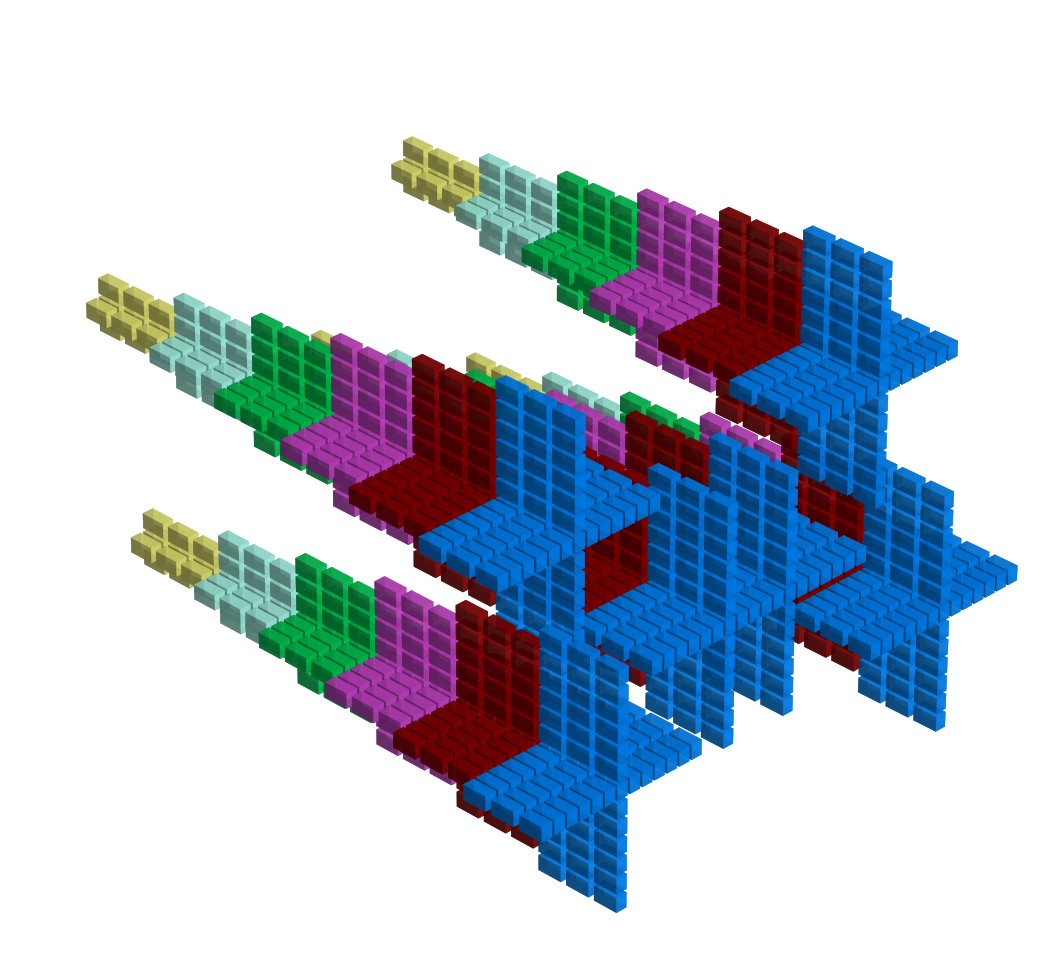
\includegraphics[width=12cm]{src/patterns/bursts/pattern0-45.png}%
    \end{adjustbox}
\caption{Evolution of the default burst at F1.}
\end{figure}
\clearpage

\begin{lstlisting}[basicstyle=\tiny,caption=Source code for the F1 Burst.]
; burstGeneratorF1
        ; currentSymmetrySetting: 'Current symmetry setting.'
        ; Possible values are 0 - 4:
        ; 'NO SYMMETRY     '
        ; 'Y-AXIS SYMMETRY '
        ; 'X-Y SYMMETRY    '
        ; 'X-AXIS SYMMETRY '
        ; 'QUAD SYMMETRY   '
        .BYTE $01
        ; smoothingDelay: 'Because of the time taken to draw larger patterns speed
        ; increase-decrease is not linear. You can adjust the compensating delay
        ; which often smooths out jerky patterns. Can be used just for special FX)
        ; though. Suck it and see.'
        .BYTE $0C

        ; Burst Position 1
        ; X/Y Co-ordinates: X/Y Position relative to cursor to place the burst.
        .BYTE $07,$06
        ; Index to pattern in pixelXPositionLoPtrArray/pixelXPositionHiPtrArray
        .BYTE $07

        ; Burst Position 2
        ; X/Y Co-ordinates: X/Y Position relative to cursor to place the burst.
        .BYTE $11,$0D
        ; Index to pattern in pixelXPositionLoPtrArray/pixelXPositionHiPtrArray
        .BYTE $07

        ; Burst Position 3
        ; X/Y Co-ordinates: X/Y Position relative to cursor to place the burst.
        .BYTE $06,$11
        ; Index to pattern in pixelXPositionLoPtrArray/pixelXPositionHiPtrArray
        .BYTE $07

        ; Burst Position 4
        ; X/Y Co-ordinates: X/Y Position relative to cursor to place the burst.
        .BYTE $FF,$0B
        ; Index to pattern in pixelXPositionLoPtrArray/pixelXPositionHiPtrArray
        .BYTE $07

        ; Burst Position 5
        ; X/Y Co-ordinates: X/Y Position relative to cursor to place the burst.
        .BYTE $FF,$00
        ; Index to pattern in pixelXPositionLoPtrArray/pixelXPositionHiPtrArray
        .BYTE $FF

        ; Burst Position 6
        ; X/Y Co-ordinates: X/Y Position relative to cursor to place the burst.
        .BYTE $21,$06
        ; Index to pattern in pixelXPositionLoPtrArray/pixelXPositionHiPtrArray
        .BYTE $00

        ; Burst Position 7
        ; X/Y Co-ordinates: X/Y Position relative to cursor to place the burst.
        .BYTE $06,$01
        ; Index to pattern in pixelXPositionLoPtrArray/pixelXPositionHiPtrArray
        .BYTE $06

        ; Burst Position 8
        ; X/Y Co-ordinates: X/Y Position relative to cursor to place the burst.
        .BYTE $41,$FF
        ; Index to pattern in pixelXPositionLoPtrArray/pixelXPositionHiPtrArray
        .BYTE $00

        ; Burst Position 9
        ; X/Y Co-ordinates: X/Y Position relative to cursor to place the burst.
        .BYTE $06,$01
        ; Index to pattern in pixelXPositionLoPtrArray/pixelXPositionHiPtrArray
        .BYTE $06

        ; Burst Position 10
        ; X/Y Co-ordinates: X/Y Position relative to cursor to place the burst.
        .BYTE $01,$06
        ; Index to pattern in pixelXPositionLoPtrArray/pixelXPositionHiPtrArray
        .BYTE $00
\end{lstlisting}

\clearpage
\begin{figure}[H]
    \centering
    \begin{adjustbox}{width=12cm,center}
      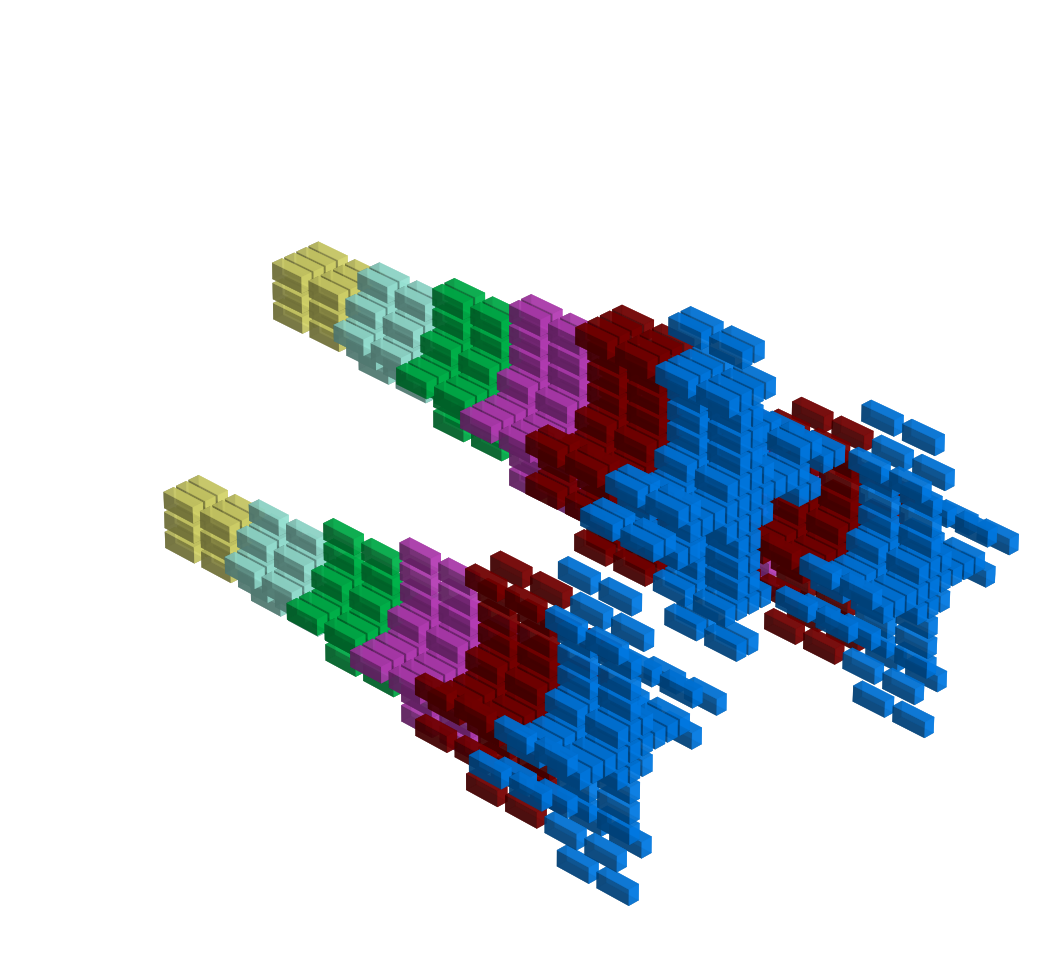
\includegraphics[width=12cm]{src/patterns/bursts/pattern1-45.png}%
    \end{adjustbox}
\caption{Evolution of the default burst at F2.}
\end{figure}
\clearpage

\begin{lstlisting}[basicstyle=\tiny,caption=Source code for the F2 Burst.]
; burstGeneratorF2
        ; currentSymmetrySetting: 'Current symmetry setting.'
        ; Possible values are 0 - 4:
        ; 'NO SYMMETRY     '
        ; 'Y-AXIS SYMMETRY '
        ; 'X-Y SYMMETRY    '
        ; 'X-AXIS SYMMETRY '
        ; 'QUAD SYMMETRY   '
        .BYTE $01
        ; smoothingDelay: 'Because of the time taken to draw larger patterns speed
        ; increase/decrease is not linear. You can adjust the compensating delay
        ; which often smooths out jerky patterns. Can be used just for special FX)
        ; though. Suck it and see.'
        .BYTE $0C

        ; Burst Position 1
        ; X/Y Co-ordinates: X/Y Position relative to cursor to place the burst.
        .BYTE $13,$08
        ; Index to pattern in pixelXPositionLoPtrArray/pixelXPositionHiPtrArray
        .BYTE $00

        ; Burst Position 2
        ; X/Y Co-ordinates: X/Y Position relative to cursor to place the burst.
        .BYTE $07,$0F
        ; Index to pattern in pixelXPositionLoPtrArray/pixelXPositionHiPtrArray
        .BYTE $00

        ; Burst Position 3
        ; X/Y Co-ordinates: X/Y Position relative to cursor to place the burst.
        .BYTE $FF,$00
        ; Index to pattern in pixelXPositionLoPtrArray/pixelXPositionHiPtrArray
        .BYTE $06

        ; Burst Position 4
        ; X/Y Co-ordinates: X/Y Position relative to cursor to place the burst.
        .BYTE $01,$2A
        ; Index to pattern in pixelXPositionLoPtrArray/pixelXPositionHiPtrArray
        .BYTE $41

        ; Burst Position 5
        ; X/Y Co-ordinates: X/Y Position relative to cursor to place the burst.
        .BYTE $02,$00
        ; Index to pattern in pixelXPositionLoPtrArray/pixelXPositionHiPtrArray
        .BYTE $04

        ; Burst Position 6
        ; X/Y Co-ordinates: X/Y Position relative to cursor to place the burst.
        .BYTE $62,$FF
        ; Index to pattern in pixelXPositionLoPtrArray/pixelXPositionHiPtrArray
        .BYTE $41

        ; Burst Position 7
        ; X/Y Co-ordinates: X/Y Position relative to cursor to place the burst.
        .BYTE $06,$40
        ; Index to pattern in pixelXPositionLoPtrArray/pixelXPositionHiPtrArray
        .BYTE $00

        ; Burst Position 8
        ; X/Y Co-ordinates: X/Y Position relative to cursor to place the burst.
        .BYTE $6B,$04
        ; Index to pattern in pixelXPositionLoPtrArray/pixelXPositionHiPtrArray
        .BYTE $41

        ; Burst Position 9
        ; X/Y Co-ordinates: X/Y Position relative to cursor to place the burst.
        .BYTE $FF,$00
        ; Index to pattern in pixelXPositionLoPtrArray/pixelXPositionHiPtrArray
        .BYTE $FF

        ; Burst Position 10
        ; X/Y Co-ordinates: X/Y Position relative to cursor to place the burst.
        .BYTE $00,$FF
        ; Index to pattern in pixelXPositionLoPtrArray/pixelXPositionHiPtrArray
        .BYTE $00
\end{lstlisting}

\clearpage
\begin{figure}[H]
    \centering
    \begin{adjustbox}{width=12cm,center}
      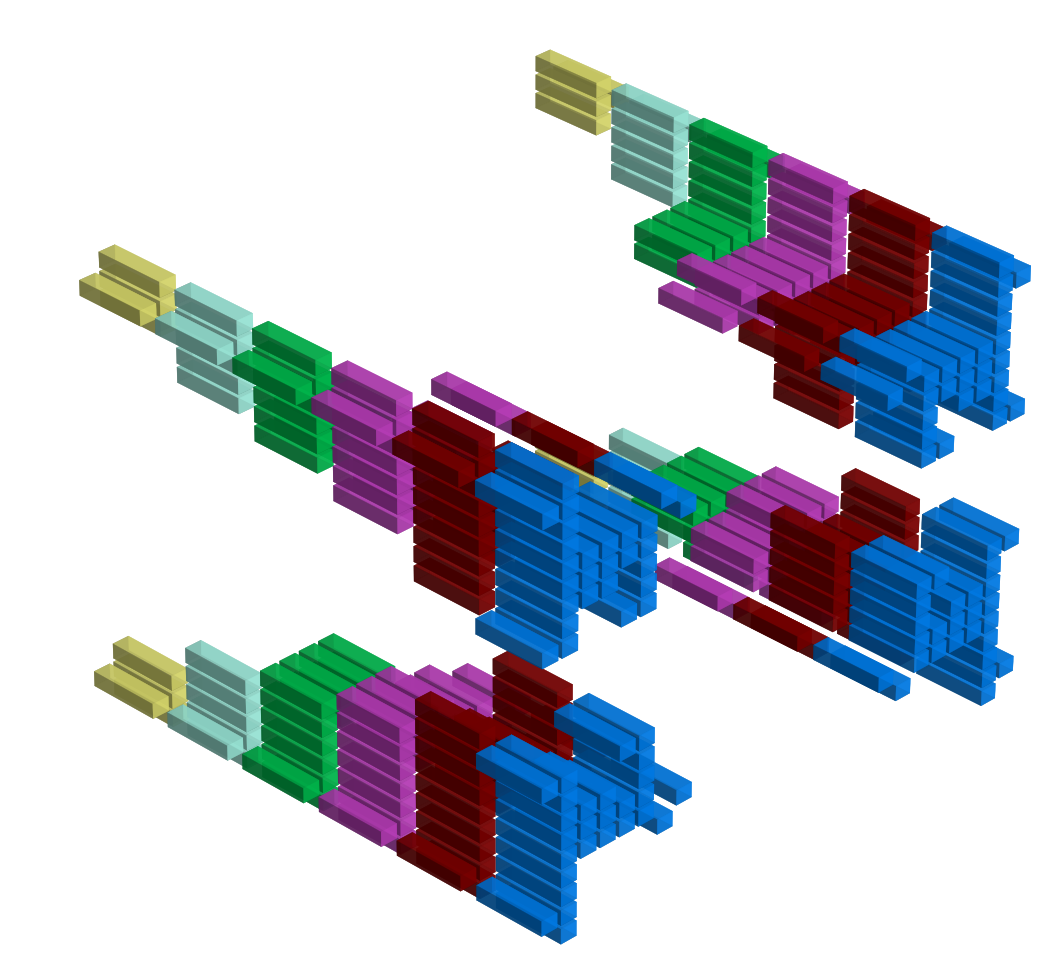
\includegraphics[width=12cm]{src/patterns/bursts/pattern2-45.png}%
    \end{adjustbox}
\caption{Evolution of the default burst at F3.}
\end{figure}
\clearpage

\begin{lstlisting}[basicstyle=\tiny,caption=Source code for the F3 Burst.]
; burstGeneratorF3
        ; currentSymmetrySetting: 'Current symmetry setting.'
        ; Possible values are 0 - 4:
        ; 'NO SYMMETRY     '
        ; 'Y-AXIS SYMMETRY '
        ; 'X-Y SYMMETRY    '
        ; 'X-AXIS SYMMETRY '
        ; 'QUAD SYMMETRY   '
        .BYTE $04
        ; smoothingDelay: 'Because of the time taken to draw larger patterns speed
        ; increase/decrease is not linear. You can adjust the compensating delay
        ; which often smooths out jerky patterns. Can be used just for special FX)
        ; though. Suck it and see.'
        .BYTE $01

        ; Burst Position 1  
        ; X/Y Co-ordinates: X/Y Position relative to cursor to place the burst.
        .BYTE $08,$01
        ; Index to pattern in pixelXPositionLoPtrArray/pixelXPositionHiPtrArray
        .BYTE $02

        ; Burst Position 2
        ; X/Y Co-ordinates: X/Y Position relative to cursor to place the burst.
        .BYTE $FF,$01
        ; Index to pattern in pixelXPositionLoPtrArray/pixelXPositionHiPtrArray
        .BYTE $02

        ; Burst Position 3
        ; X/Y Co-ordinates: X/Y Position relative to cursor to place the burst.
        .BYTE $08,$01
        ; Index to pattern in pixelXPositionLoPtrArray/pixelXPositionHiPtrArray
        .BYTE $02

        ; Burst Position 4
        ; X/Y Co-ordinates: X/Y Position relative to cursor to place the burst.
        .BYTE $08,$01
        ; Index to pattern in pixelXPositionLoPtrArray/pixelXPositionHiPtrArray
        .BYTE $02

        ; Burst Position 5
        ; X/Y Co-ordinates: X/Y Position relative to cursor to place the burst.
        .BYTE $08,$01
        ; Index to pattern in pixelXPositionLoPtrArray/pixelXPositionHiPtrArray
        .BYTE $02

        ; Burst Position 6
        ; X/Y Co-ordinates: X/Y Position relative to cursor to place the burst.
        .BYTE $08,$01
        ; Index to pattern in pixelXPositionLoPtrArray/pixelXPositionHiPtrArray
        .BYTE $02

        ; Burst Position 7
        ; X/Y Co-ordinates: X/Y Position relative to cursor to place the burst.
        .BYTE $08,$01
        ; Index to pattern in pixelXPositionLoPtrArray/pixelXPositionHiPtrArray
        .BYTE $02

        ; Burst Position 8
        ; X/Y Co-ordinates: X/Y Position relative to cursor to place the burst.
        .BYTE $FF,$03
        ; Index to pattern in pixelXPositionLoPtrArray/pixelXPositionHiPtrArray
        .BYTE $02

        ; Burst Position 9
        ; X/Y Co-ordinates: X/Y Position relative to cursor to place the burst.
        .BYTE $08,$03
        ; Index to pattern in pixelXPositionLoPtrArray/pixelXPositionHiPtrArray
        .BYTE $02

        ; Burst Position 10
        ; X/Y Co-ordinates: X/Y Position relative to cursor to place the burst.
        .BYTE $08,$03
        ; Index to pattern in pixelXPositionLoPtrArray/pixelXPositionHiPtrArray
        .BYTE $02
\end{lstlisting}

\clearpage
\begin{figure}[H]
    \centering
    \begin{adjustbox}{width=12cm,center}
      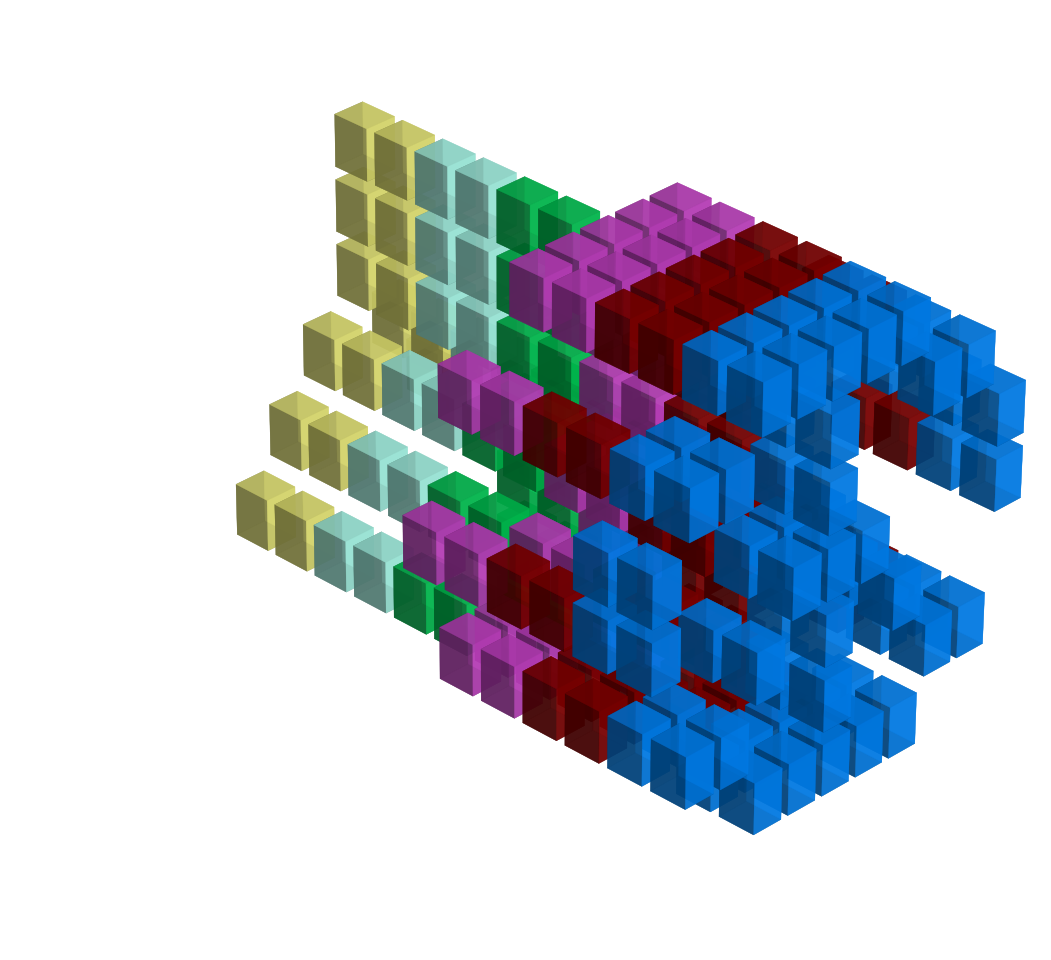
\includegraphics[width=12cm]{src/patterns/bursts/pattern3-45.png}%
    \end{adjustbox}
\caption{Evolution of the default burst at F3.}
\end{figure}
\clearpage

\begin{lstlisting}[basicstyle=\tiny,caption=Source code for the F3 Burst.]
; burstGeneratorF4
        ; currentSymmetrySetting: 'Current symmetry setting.'
        ; Possible values are 0 - 4:
        ; 'NO SYMMETRY     '
        ; 'Y-AXIS SYMMETRY '
        ; 'X-Y SYMMETRY    '
        ; 'X-AXIS SYMMETRY '
        ; 'QUAD SYMMETRY   '
        .BYTE $00
        ; smoothingDelay: 'Because of the time taken to draw larger patterns speed
        ; increase/decrease is not linear. You can adjust the compensating delay
        ; which often smooths out jerky patterns. Can be used just for special FX)
        ; though. Suck it and see.'
        .BYTE $11

        ; Burst Position 1
        ; X/Y Co-ordinates: X/Y Position relative to cursor to place the burst.
        .BYTE $12,$09
        ; Index to pattern in pixelXPositionLoPtrArray/pixelXPositionHiPtrArray
        .BYTE $08

        ; Burst Position 2
        ; X/Y Co-ordinates: X/Y Position relative to cursor to place the burst.
        .BYTE $12,$09
        ; Index to pattern in pixelXPositionLoPtrArray/pixelXPositionHiPtrArray
        .BYTE $08

        ; Burst Position 3
        ; X/Y Co-ordinates: X/Y Position relative to cursor to place the burst.
        .BYTE $FF,$08
        ; Index to pattern in pixelXPositionLoPtrArray/pixelXPositionHiPtrArray
        .BYTE $03

        ; Burst Position 4
        ; X/Y Co-ordinates: X/Y Position relative to cursor to place the burst.
        .BYTE $02,$08
        ; Index to pattern in pixelXPositionLoPtrArray/pixelXPositionHiPtrArray
        .BYTE $03

        ; Burst Position 5
        ; X/Y Co-ordinates: X/Y Position relative to cursor to place the burst.
        .BYTE $02,$08
        ; Index to pattern in pixelXPositionLoPtrArray/pixelXPositionHiPtrArray
        .BYTE $03

        ; Burst Position 6
        ; X/Y Co-ordinates: X/Y Position relative to cursor to place the burst.
        .BYTE $02,$FF
        ; Index to pattern in pixelXPositionLoPtrArray/pixelXPositionHiPtrArray
        .BYTE $00

        ; Burst Position 7
        ; X/Y Co-ordinates: X/Y Position relative to cursor to place the burst.
        .BYTE $00,$00
        ; Index to pattern in pixelXPositionLoPtrArray/pixelXPositionHiPtrArray
        .BYTE $00

        ; Burst Position 8
        ; X/Y Co-ordinates: X/Y Position relative to cursor to place the burst.
        .BYTE $01,$24
        ; Index to pattern in pixelXPositionLoPtrArray/pixelXPositionHiPtrArray
        .BYTE $00

        ; Burst Position 9
        ; X/Y Co-ordinates: X/Y Position relative to cursor to place the burst.
        .BYTE $05,$01
        ; Index to pattern in pixelXPositionLoPtrArray/pixelXPositionHiPtrArray
        .BYTE $00

        ; Burst Position 10
        ; X/Y Co-ordinates: X/Y Position relative to cursor to place the burst.
        .BYTE $00,$00
        ; Index to pattern in pixelXPositionLoPtrArray/pixelXPositionHiPtrArray
        .BYTE $00

\end{lstlisting}

